\chapter{Developing a language}\label{ch:TheCompiler}
In this chapter we will take a look at what needs to be done in order to create a language. First of all, a compiler needs to be built, and thus a short introduction to this will be presented together with how the syntax analysis is done for a language. Finally, we will examine the definition of the syntax and functionality of the language. 
\section{The compiler}
A compiler is essentially a program which takes a source code in one language as input, and then converts this to have the same properties in another target language as output. The compiler we are to build, must be able to compile programs written in PHAL into APL which will then be further compiled into a .hex file which is executable by an Arduino machine\cite{ArduinoBuildProcess}.
\subsection{Compilation phases}
When compiling a program, the source code has to go through a number of compilation phases before the target code can be generated. These phases consist of:
\begin{itemize}
    \item Scanning
    \item Parsing
    \item Creation of the abstract syntax tree (AST)
    \item Semantic analysis of the AST
    \item Traversal of the AST to generate translation
\end{itemize}
\begin{figure}[H]
\centering
  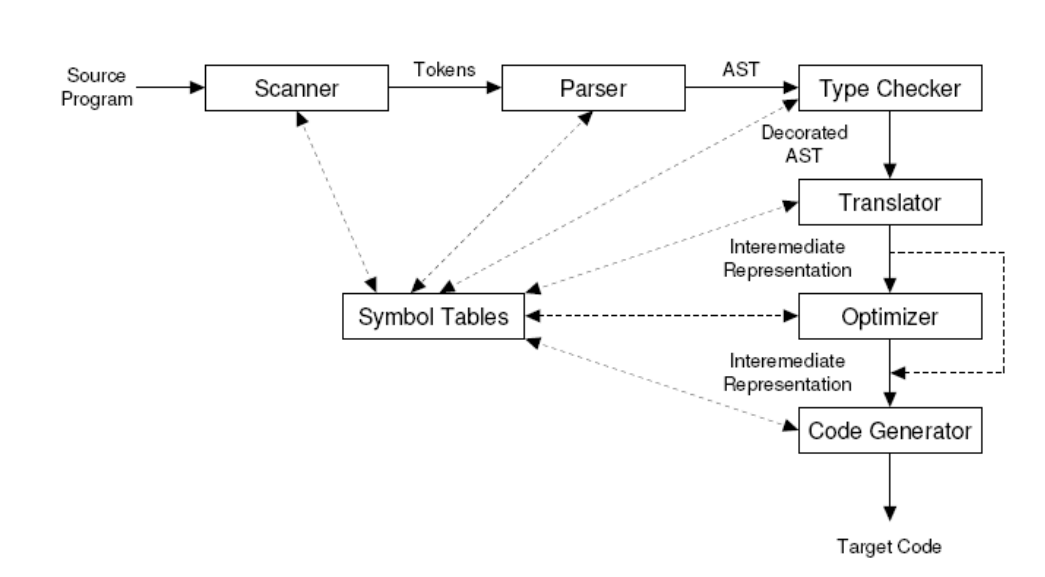
\includegraphics[scale=0.5]{figures/CompilerPhases/compilerPhases.PNG}
  \caption{This figure shows a syntax-directed compiler \cite{CraftinfACompiler}. }
  \label{fig:compilerPhases}
\end{figure}
\noindent
On Figure~\ref{fig:compilerPhases} the phases which the compilation process goes through is shown. Firstly, the source program written by a programmer in a specific language is used as input. This is then analysed, where each string of the input is scanned and sorted into different categories of strings called \textit{tokens}. These tokens are then syntactically analysed in the parser to check if the code submits to the rules defined in the grammar for the language. After the syntactic analysis has constructed the abstract syntax tree, as shown on figure \ref{fig:compilerPhases}, the semantic analysis takes place. During this phase the code is semantically checked, meaning that types and scopes are identified and defined. If the source code passes these different phases, the target code can be generated, which is the final phase of the compiler \cite{CraftinfACompiler}.
 
\section{Syntax analysis}
In this section we take a look at the different parts of the syntax analysis. The syntax analysis is the first part of the compilation phase, and it is responsible for making sure that the compiler can recognise the language that has been defined with the grammar. 
% Chapter 3 Fischer
\subsection{Lexical analysis - the scanner}
The scanner is responsible for looking through all of the characters in the source code and find tokens in the code. This is known as the lexical analysis, which is the first part of the syntax analysis. 
\\\\
The scanner will often be able to look a few characters ahead which helps determine what kind of token it is reading. If the scanner finds input that is not part of a defined token, it should show an error. The output of the scanner is a more compact version of the source code, which is represented as a stream of tokens. The scanner will simplify the job of the \textit{parsers} by eliminating the unneeded information, such as whitespace, and by sorting the source code into tokens \cite{CraftinfACompiler} rather than source code.
\\\\
\textbf{Tokens}
\\\\
Tokens are different categories of specific strings that have been sorted by the lexical analyser. A token can, for example, be identifiers, integers or reserved words. The reason that the string of characters which are input to the lexical analyser must be sorted into tokens, is to make it possible for the parser to check if the input is correctly written in relation to the defined grammar.
\\\\
\textbf{Regular expressions}
\\\\
The scanner needs a method to recognise which category of tokens the strings belong to. To do this, the scanner uses regular expressions to look for the tokens. Regular expressions describe the alphabet that a token consists of, and how the characters of the alphabet can be put together to form a string that belongs to this token. For example an integer is expressed as:
\begin{center}
    ( \{-\} ? \{1-9\} \{0-9\}* ) $\cup$ \{0\}
\end{center}
This regular expression shows that an integer can be preceded by zero or one \textit{"-"} which is indicated with the \textit{?} operator, followed by an integer between 1 and 9, and then zero or more integers between 0 and 9 which is indicated with the \textit{*}. The integer can also just be a single 0. Regular expressions for types in PHAL will be described further in chapter \ref{FormalDefinition}
\\\\
\textbf{Finite automata}\
\\\\
Regular expressions are a convenient notation for describing tokens in programming languages. This is due to regular expressions being able to be converted into nondeterministic finite state automatons (NFAs), which can be converted into deterministic finite state automatons (DFAs). This is useful as DFAs can be easily implemented as computer programs. 
\\\\
The finite state automaton is defined by Michael Sipser in the book \textit{Introduction to the Theory of Computation} as a 5-tuple consisting of the following:
\begin{itemize}
    \item \textit{Q} is a finite set called the \textit{states}
    \item $\Sigma$ is a finite set called the \textit{alphabet}, which is any non-empty finite set 
    \item $\delta$: $Q$ $\times$ $\Sigma \xrightarrow{}$ $Q$ is the \textit{transition function} which defines the rules for moving between states, where the domain of the function is the set $Q$ $\times$ $\Sigma$ and the range is $Q$
    \item $q_{0}$ $\in$ \textit{Q} is the \textit{start state}, meaning the start state is found in the set of states \textit{Q}
    \item \textit{F} $\subseteq$ \textit{Q} is the \textit{set of accept states}, meaning the set \textit{F} of accept states is a subset of \textit{Q} \cite{sipser}
\end{itemize}
Below is an example of a DFA:
\begin{figure}[H]
\centering
  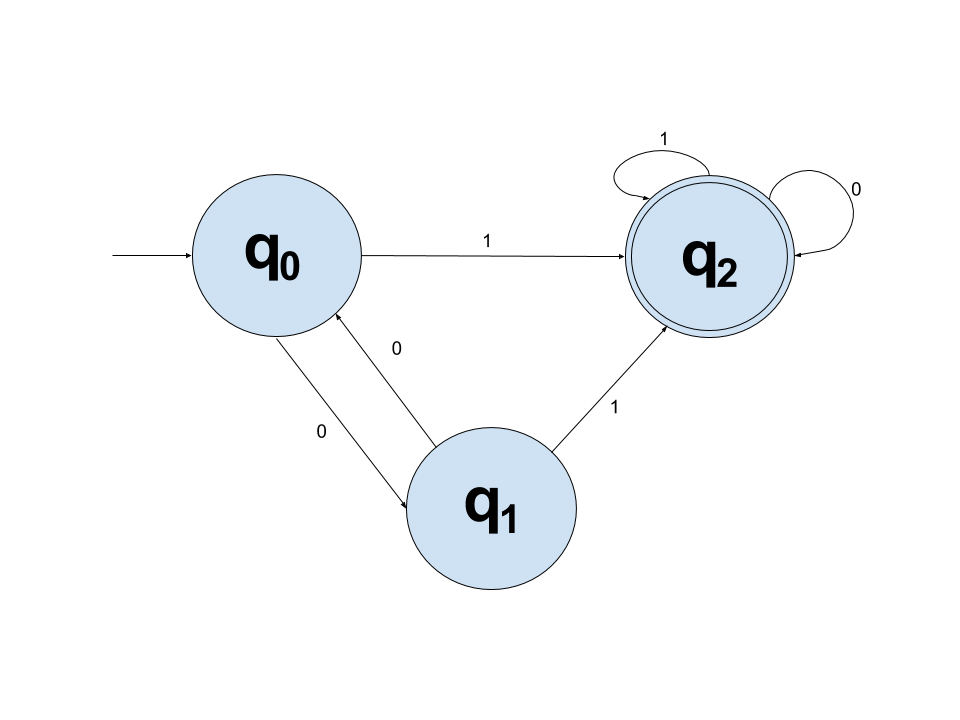
\includegraphics[scale=0.35]{figures/DFA.png}
  \caption{This figure shows an example of a DFA.}
  \label{fig:dfaExample}
\end{figure}
\noindent
In this example, the states are $Q = \{q0, q1, q2\}$, the alphabet is $\Sigma = \{0,1\}$, the start state $q_{0}$ is $q0$ and the accept state $F$ is $q2$. 
The arrows show how the automaton transitions from one state to another when it receives a given input. 
$q2$ is the accept state, this automaton accepts any string that contains a $1$ , no matter how many times it appears or where in the string it appears. 
This is shown by the transitions from states $q0$ and $q1$ to the accept state requiring a $1$, and the iterations in the accept state that do not allow the input to transition away from the accept state. 
This automaton is deterministic, as there is always only one choice for a transition to a new state for a given input. 
\\\\
In a non-deterministic finite automaton (NFA), it could be possible to choose two transitions from a single state with one input. 
For example in figure \ref{fig:dfaExample}, if the transition from state $q0$ to state $q1$ was defined by a transition requiring $1$ as input, the automaton would be able to transition to both state $q1$ and state $q2$, making it non-deterministic. 
\\\\
This ultimately means that the generation of a scanner is based on:
\begin{itemize}
    \item Regular expressions to describe the tokens to be recognised
    \item Finite state automatons as an execution model to which regular expressions are "compiled"
\end{itemize}
% Write more about regular expressions?

\subsection{Syntactic analysis - the parser}
% Chapter 4 FISCHER
The parser is the part of the compiler responsible for checking if the tokens that are provided by the scanner fit the grammar specification for the language. This is where the \textit{Context-Free-Grammar} (CFG) is introduced, because the parser has to check the syntax of the language using the CFG as reference. 

\subsubsection{Context-Free-Grammars}
Context-Free-Grammars are a set of grammar rules/productions that define the grammar of the language. 
A CFG consists of terminal and non-terminal symbols. 
Terminal symbols represent strings that can be derived to a token category. 
The non-terminal symbols all define a production on their right-hand-side. 
\begin{lstlisting}[caption={Example of an Context-Free-Grammer}, label={example:cfg}]
Prog    -> A B C
A       -> a
B       -> d e A
        |  b
C       -> c

\end{lstlisting}
On Listing~\ref{example:cfg} a short example of a CFG can be seen. 
The first rule says that a non-terminal symbol \textit{Prog} can be derived to the non-terminal symbols \textit{A B C}. 
Non-terminal symbols all start with a capital letter. 
\\
As seen on line 3 on Listing~\ref{example:cfg} the non-terminal \textit{B} has two productions, meaning it can either be derived to \textit{d e A} or \textit{b}.
Terminal symbols on the other hand can not derive further. 
It should be possible to create a sentence containing only terminal symbols which can then be replaced by tokens \cite{CraftinfACompiler}.
An example of this, using the CFG specified on Listing~\ref{example:cfg} is shown in Listing~\ref{example:cfgderive}.
On the final line it is seen that all non-terminals has been derived to terminal symbols.
\begin{lstlisting}[caption={Example of an Context-Free-Grammer derivation}, label={example:cfgderive}]
Prog
=> A B C                ( Prog  -> A B C )
=> a B C                ( A     -> a)
=> a d e A C            ( B     -> d e A)
=> a d e a C            ( A     -> a)
=> a d e a c            ( C     -> c) 
\end{lstlisting}

\subsubsection{Recursive descent}
Recursive descent is a simple parsing technique used for parsers. 
In recursive descent, each non-terminal from the CFG is a procedure. 
The procedure then examines the next token from the token stream, provided by the scanner, to evaluate which production should be used. 
If there is a non-terminal on the right-hand-side, the procedure calls the procedure for this particular non-terminal, and thus we have the recursive part of the technique, because the procedure goes through the derivation tree for the stream of tokens.
\\\\
For example, if we look at the short CFG shown on Listing~\ref{example:cfg}, the procedure for the non-terminal \textit{B} would be represented as shown in Listing~\ref{RD:Procedure}. 
\begin{lstlisting}[caption={Procedure for a recursive descent of the CFG productions}, label={RD:Procedure}]
procedure B()
  if ts.peek()= d
  then
    call match(ts,d)
    call match(ts,e)
    call A()
  else
    if ts.peek()= b
    then
      call match(ts,b) 
    else
      call error()
end
\end{lstlisting}
As seen on Listing~\ref{RD:Procedure}, the procedure for \textit{B} needs to look for which production is being used. 
If it peeks \textit{d} on line 2, it expects to see \textit{d} followed by an \textit{e}, and then calls the procedure for the non-terminal \textit{A}. 
Otherwise if it peeks a \textit{b}, the procedure expects the terminal token \textit{b} and nothing else. 
If what the procedure peeks are neither \textit{d} nor \textit{b} an error will be called.
\\\\
To complete the recursive descent parser, a procedure like this has to be written for each of the non-terminals in the CFG, where every possible production has to be considered.
\\\\
Once the lexer and the parser phases are complete, the compiler is able to recognise text that is written in the specified language in accordance with the grammar. 
These two phases are only responsible for the syntactical analysis part of the compilation. 
\\\\
The compiler still does not understand if the correct types are used for the various expressions for example. 
Type checking and code generation must still be done by the compiler before it can be considered complete.

\section{Contextual analysis}\label{comp:ContextualA}
%% Skrevet fra chapter 2.7
After the source code has been through the syntax analysis by the parser and the abstract syntax tree has been generated, it is time for the contextual analysis. In this phase the source code is checked for aspects that are not easily seen by the syntax analysis, such as checking that identifiers are declared before use, the scope of the variables and type-checking using a symbol table. 
\subsubsection{Symbol tables}
In many languages, it is a requirement that identifiers are declared before use. This is also a requirement in PHAL, and to enforce this requirement a symbol table is used. The symbol table is created by traversing the AST and looking for identifiers, which are then written to the symbol table along with their type. Other things that are usually stored together with the identifiers are their scope, their storage class and their protection properties.

\subsubsection{Type checking}
Type checking is part of the semantic analysis, and the symbol table is used to check for type consistency. 
%% type hierarchy?
Many languages have a type hierarchy where for example a float is considered \textit{wider} than an int, because an int can be represented as a float, but not the other way around. So converting an int to float is often done automatically, but a float number to int has to be done explicitly, because the number loses precision in the conversion.
\\\\
The general process known as type checking consists of traversing the AST bottom-up, meaning that it goes from the leaves of the tree to the root. There are different approaches that can be used to traverse the AST, and one that is often used is the \textit{visitor pattern}. This pattern can be used to determine what the calculated type of a statement is, based on what is in the AST. 

\subsubsection{Visitor pattern}\label{comp:VisitorPattern}
To traverse the AST, the visitor pattern can be used. 
The visitor is class that has different methods for each type of object it will visit during the traversal. 
The \textit{Visitor} class will often be used as the super class and the derived class will then override methods where extra functionality is needed.
%Each operation that can be used is implemented as a subclass of the general visitor class. 
\\\\
The nodes that are operated on accepts the visitor and calls back the appropriate type-specific method using themselves as the parameters. 
This means new operations can be added without modifying the object types, meaning you would implement a new visitor rather than changing the given class for the specific node. 
The visitors implement the operations and have one method for each type of node they visit. 
\\\\
Ultimately, this means the visitor pattern is the super class of classes such as \textit{TypeChecker} and \textit{CodeGenerator} that implement the \textit{Visitor} abstract class, and all the AST node classes have \textit{accept} methods that call back the appropriate method.

\subsubsection{Decorated abstract syntax tree}
The decorated abstract syntax tree (DAST) is the result of the contexual analysis. The DAST is an AST that is annotated with useful information, such as the position in the source code, which can be used for error reporting, and the types that will be used for the semantic analysis.
\\
After this, the final part of the compilation is the code generation of the target language. In the code generation phase the decorated abstract syntax tree is used to generate the correct instruction based on the types. 
\\
The individual phases will be further described in Part~III  about compiler design.